\documentclass[10pt,a4paper]{report}

% packages
\usepackage[utf8]{inputenc}
\usepackage{mathrsfs}
% used for: \mathscr{Q}
\usepackage{amsmath}
\usepackage{dsfont}
% used for: \mathds{E}
\usepackage{svg}
\usepackage{float}
\usepackage{rotating}

% \usepackage{layouts}

% 
\newcounter{example}[section]
\newenvironment{example}[1][]{\refstepcounter{example}\par\medskip\noindent\textbf{Example~\theexample. #1}\rmfamily}{\medskip}

% definitions
\DeclareMathOperator*{\argmin}{arg\,min}
\DeclareMathOperator{\KL}{KL}
\DeclareMathOperator{\ELBO}{ELBO}

% http://detexify.kirelabs.org/classify.html

\begin{document}

\title{Modelling single-cell RNA-seq data using variational Autoencoders}
\author{Andrej Balaz}
\date{\today}
\maketitle

% \begin{abstract}
% The abstract will be here...
% \end{abstract}

\tableofcontents
%\listoffigures
%\listoftables
\newpage

\chapter{Introduction}
\label{chap:intro}

% What is single-cell RNA sequencing
Single-cell RNA sequencing is an important tool for analysing the biological processes in the fields such as oncology, developmental biology, neurology, and study of autoimmune and infectious diseases \cite{patel2014single}.
In comparison with its older cousin, bulk RNA sequencing, it provides us with the expression profile at a resolution of individual cells.
In spite of the impossibility of retrieving the full information of the expression profile due to the small number of transcripts in a particular cell, this data can be used to find the patterns of gene expression \cite{lopez2018scvi}.
Using clustering analysis on these high-resolution patterns, we can uncover rare cell types, never observed in the tissue before.
% What are the biases in the single-cell RNA-seq experiment and how do they arise?
However, the interpretation of the single-cell RNA-seq data remains challenging, mainly because of the high dimensionality of such data, limited and variable sensitivity, batch effects and transcriptional noise.
% Modelling of the single-cell RNA-seq data can be used for various tasks such as imputations of missing values, clustering of the different cells and differential expression analysis.
% What was done up to this point?
Several methods have been proposed for this task \cite{pierson2015zifa}.
Unfortunately, most of these methods assume that a generalized linear model can be used to map the single-cell RNA-seq data to a low dimensional representation.
Furthermore, most existing methods cannot be applied to recent huge datasets consisting of many thousands of cells \cite{regev2017science}.

% What will we try to achieve in this work?
In this report, we explore the possibility to model single-cell data by using the variational autoencoder.
This approach allows us to use a non-linear function to map the data to its low dimensional representation.
Furthermore, this representation is probabilistic, which allows us to model the uncertainty of our representation, which might be important information for the downstream analysis.
Also, after the training phase, our model can be used to quickly evaluate new data, which makes it suitable for huge datasets.
% A special type of neural network, which allows us to map single-cell DNA to lower-dimensional latent space.

To introduce variational autoencoder, we need to define and explain a lot of new terminologies.

First, we briefly introduce the concept of neural networks with special attention to autoencoders, because this is the basic machine learning model we are extending in variational autoencoder.

Since our model creates a probabilistic representation, we need to explain the basics of bayesian modelling.
To illustrate the main goal of approximate Bayesian inference, we use the approximate Bayesian computation, because this method is easy to understand.
Other methods aim for the same goal but are using some clever tricks to get there faster.
Next, we compare the most commonly used methods, Markov chain Monte Carlo, to variational inference used in this project and explain the variational inference in details.
Finally, we show how to merge the two concepts of variational inference and autoencoder into variational autoencoder.

% We start by introducing the basics of variational inference and compare it to the classical Bayesian approach.
Afterwards, we present the model created in this project and we show the experiments we performed on well-known MNIST dataset \cite{lecun1998gradient} to test the correctness of our implementation.
Finally, we demonstrate how to use the model on the single-cell RNA-seq data.

\chapter{Methods}
\label{chap:methods}

In this chapter we will describe the process of variational inference and compare it to markov chain monte carlo methods (MCMC).
We describe the basics of autoencoders architecture.
Next we combine these two to variational autoencoder.

\section{Variational inference}
The main idea behind variational inference is to use optimization.
First, we posit a family of approximate densities $\mathscr{Q}$. \cite{blei2017statreview} 

Then, we try to find the member of that family that minimizes the Kullback-Leibler(KL) divergence to the exact posterior,
$$q^{\ast}(z) = \argmin_{q(z) \in \mathscr{Q}} \KL(q(z) \| p(z|x))$$.
Finally, we approximate the posterior with the optimized member of the family $q^{\ast}(\cdot)$.

$$p(z|x)=\frac{p(z,x)}{p(x)}$$

The denominator, sometimes called the evidence, is intractable.

The goal:
$$
q^{\ast}(z) = \argmin_{q(z) \in \mathscr{Q}} \KL(q(z) \| p(z|x))
$$

$$
- \KL(q(z) \| p(z|x)) = - \mathds{E}[\log q(z)] + \mathds{E}[\log p(z,x)] - \log p(x).
$$
Because we cannot compute the $KL$, we optimize an alternative objective that is equivalentto the $KL$ up to an added constant,
$$
\ELBO(q) = \mathds{E}[\log p(z,x)] - \mathds{E}[\log q(z)]
$$

Maximizing the $\ELBO$ is equivalent to minimizing the $\KL$ divergence.
Another characteristic of $\ELBO$ is that it bounds the log evidence
$$ \log p(x) \geq \ELBO(q) $$

$$ \log p(x) = \KL( q(z) \| p(z|x)) + \ELBO(q) $$

\section{Autoencoders}
\section{Variational Autoencoders}
\chapter{Implementation}
\label{chap:results}

In this chapter, we show how we implemented variational autoencoder.
We used two different datasets to do experiments with our variational autoencoder.
The first dataset, MNIST \cite{lecun1998gradient}, is a well-known dataset used to test the implementation of new machine learning methods.
The second dataset, CORTEX \cite{lopez2018scvi}, is a single-cell RNA-seq dataset used to illustrate how the variational autoencoder can be used for the analysis of such data.

\section{MNIST variational autoencoder}

% description of the dataset
The MNIST (Modified National Institute of Standards and Technology) dataset is a set of 70000 samples.
Each sample is a picture of a hand-written digit from 0 to 9.
The pictures are represented as $28\times28$ pixels, where each pixel takes values from 0 to 255.
These values represent different shades of grey from black, represented by 0, to white, represented by 255.
Furthermore, the size of the digits is normalized and the digits are centred to the fixed-size picture.

Enormous resources have been used to collect, preprocess and label this dataset, which makes it one of the most widely used datasets for testing purposes.
The example from this dataset is shown in Figure \ref{fig:MNIST_ex}.

\begin{figure}[H]
    \centering
    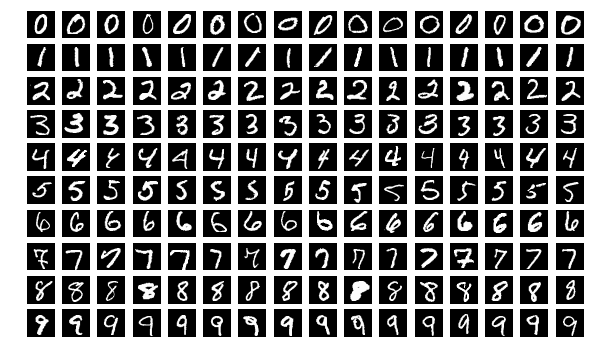
\includegraphics[scale=0.3]{images/MnistExamples.png}
    \caption{Example of the MNIST dataset}
    \label{fig:MNIST_ex}
\end{figure}

\subsection{Data preprocessing}
Since the pictures were in the form of matrices and our method took vectors as an input, we decided to flatten the data.
Therefore, we transformed each picture of $28\times28$ pixels to one vector of the size $784$.

Despite the exhaustive preprocessing of the MNIST dataset, we encountered a problem of exploding gradients using the raw data.
This problem caused that during the training certain weights became of the type NaN (not a number) and the program crashed.
Our hypothesis why this happened is mainly based on the impossibility to express very small numbers in computers.
We suspect that some probabilities close to zero were cast to zero, which then caused division by zero in the model.
Due to the non-deterministic nature of this error and relatively straightforward solution, we decided not to investigate this error further for the sake of time.

The solution to this problem was to rescale the data.
For the rescaling, we used column-wise min-max normalization given by the Equation \ref{eq:minmax}.
Furthermore, it was observed in practice that the neural networks tend to learn faster when the mean of each predictor is zero, therefore we decided to shift the scaled values accordingly. 

\begin{equation}
    x = \frac{x - min(x)}{max(x) - min(x)}
    \label{eq:minmax}
\end{equation}

% Exploding gradient and how to fight it: softplus, lower learning rate, batch normalization, fudge factor, gradient clipping, weight regularization

% details of the variational autoencoder
\subsection{Details of the variational autoencoder}
We implemented the variational autoencoder using the PyTorch library \cite{paszke2017automatic}.
The library provided us with the basic matrix operations, non-linear transformations, parametrizable probability distributions and automatic differentiation for computing the necessary gradients.

As suggested by the theory, we split the VAE to the probabilistic encoder and the probabilistic decoder.

The probabilistic encoder was a neural network with one hidden layer.
The size of the input layer was determined by the size of the input data.
The hidden layer consisted of 400 neurons with the Relu activation function used for a non-linearity.
Activations from the hidden layer were then used to feed two parallel output layers.
These output layers produced two vectors of size 20 per each, representing the variational parameters of the model.
We chose the family of all multivariate normal distributions without any covariance structure to represent the density over latent variables $z$.
Therefore, the first vector represented means of the multivariate normal distribution of the latent variable $z$ and the second vector represented log-variances of the multivariate normal distribution of the latent variable $z$.
The log-variances were used because the numbers produced by the encoder could possibly be from the interval from minus infinity to plus infinity, but the variance is defined only on non-negative values.

The two vectors were then used in the reparametrization trick.
We transformed the vector of log-variances to the vector of standard deviations.
The vector of means and the vector of standard deviations were used to define the multivariate normal distribution of the latent variable $z$.
Then, we sampled three realizations from the aforementioned multivariate normal distribution.

We used the realizations as an input to our probabilistic decoder.
The probabilistic decoder was a neural network with one hidden layer, similarly to the encoder.
Since the input was a vector of 20 values representing the latent variable $z$, the input layer consisted of 20 neurons.
These values were fed to the hidden layer with 400 neurons with the Relu activation function.
Again, activations from this hidden layer were used as an input to two parallel output layers, producing two vectors of the same size as the input data.
These vectors represented the mean and the log-variance of another multivariate normal distribution, which, we assumed, created the input data.

The visualization of the architecture is displayed in Figure \ref{fig:VAE}.

% linewidth: \printinunitsof{cm}\prntlen{\linewidth}

\begin{figure}[H]
    \centering
    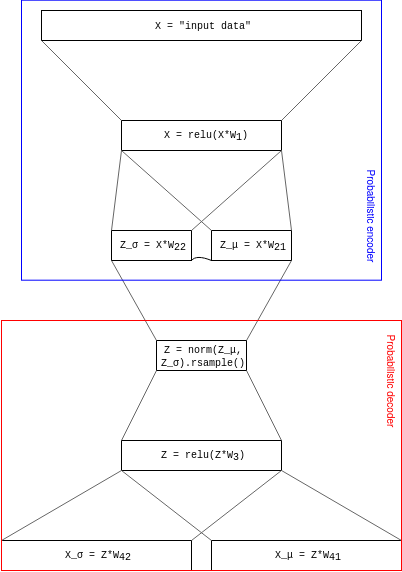
\includegraphics[width=12cm, height=15cm]{images/VAE_final.png}
    \caption{The visualization of the variational autoencoder architecture.}
    \label{fig:VAE}
\end{figure}

% the SGVB estimate
\subsection{Training of the variational autoencoder}
The training of the parameters of the variational autoencoder was done using the mini-batch stochastic gradient descent algorithm.
As error measure for optimizations, we selected the Stochastic Gradient Variational Bayes (SGVB) from the Equation \ref{eq:SGVB_b} and combined it with the Equation \ref{eq:SGVB_mb}.
Because we used a multivariate normal distribution without any covariance structure to approximate the posterior $p(z|x)$, we were able to use the analytical result for the KL divergence term.
This gave us an error measure as shown in the Equation \ref{eq:SGVB_applied}.

\begin{equation}
\begin{split}
    \widetilde{\mathcal{L}}(\theta, \phi; X^M) &= \frac{N}{M} \sum_{i=1}^{M} (-\KL(q_{\phi}(z|x_i) \| p_{\theta}(z)) + \frac{1}{L}\sum_{l=1}^{L} \log p_{\theta}(x_i|g_{\phi}(\epsilon_{il}, x_i))) \\
    &= \frac{N}{M} \sum_{i=1}^{M} (
     \frac{1}{2}\sum_{j=1}^{J}(1 + \log((\sigma_{ij})^2) - (\mu_{ij})^2 - (\sigma_{ij})^2) \\
    &\hspace{1.2cm}+\frac{1}{L}\sum_{l=1}^{L} \log p_{\theta}(x_i|g_{\phi}(\epsilon_{il}, x_i)))
\end{split}
\label{eq:SGVB_applied}
\end{equation}

The term $\mu$ corresponds to the vector of means from the probabilistic encoder network.
Similarly, the term $\sigma$ corresponds to the vector of standard deviations and can be obtained by a simple transformation $\sigma = e^{1/2\cdot logvar}$ from the vector of log-variances from the probabilistic encoder network.

To get the last term of the Equation \ref{eq:SGVB_applied}, we create a univariate normal distribution with the parameters as they are produced by the probabilistic decoder network. We can then use the original data point $x_i$ and the PyTorch's method to get the log-probability of $x_i$.

To ensure the correctness of the implementation we split the dataset to training and validation set.
We monitored the training and the validation negative SGVB quantity as shown in the Figure \ref{fig:train_test_error}.
As we expected, the training SGVB quantity decreased over time, as the variational autoencoder learned more efficient representations of the data.
Around the 80th epoch, the validation SGVB started to diverge from the training SGVB due to overfitting of the model, therefore we stopped the training.

\begin{figure}[H]
    \centering
    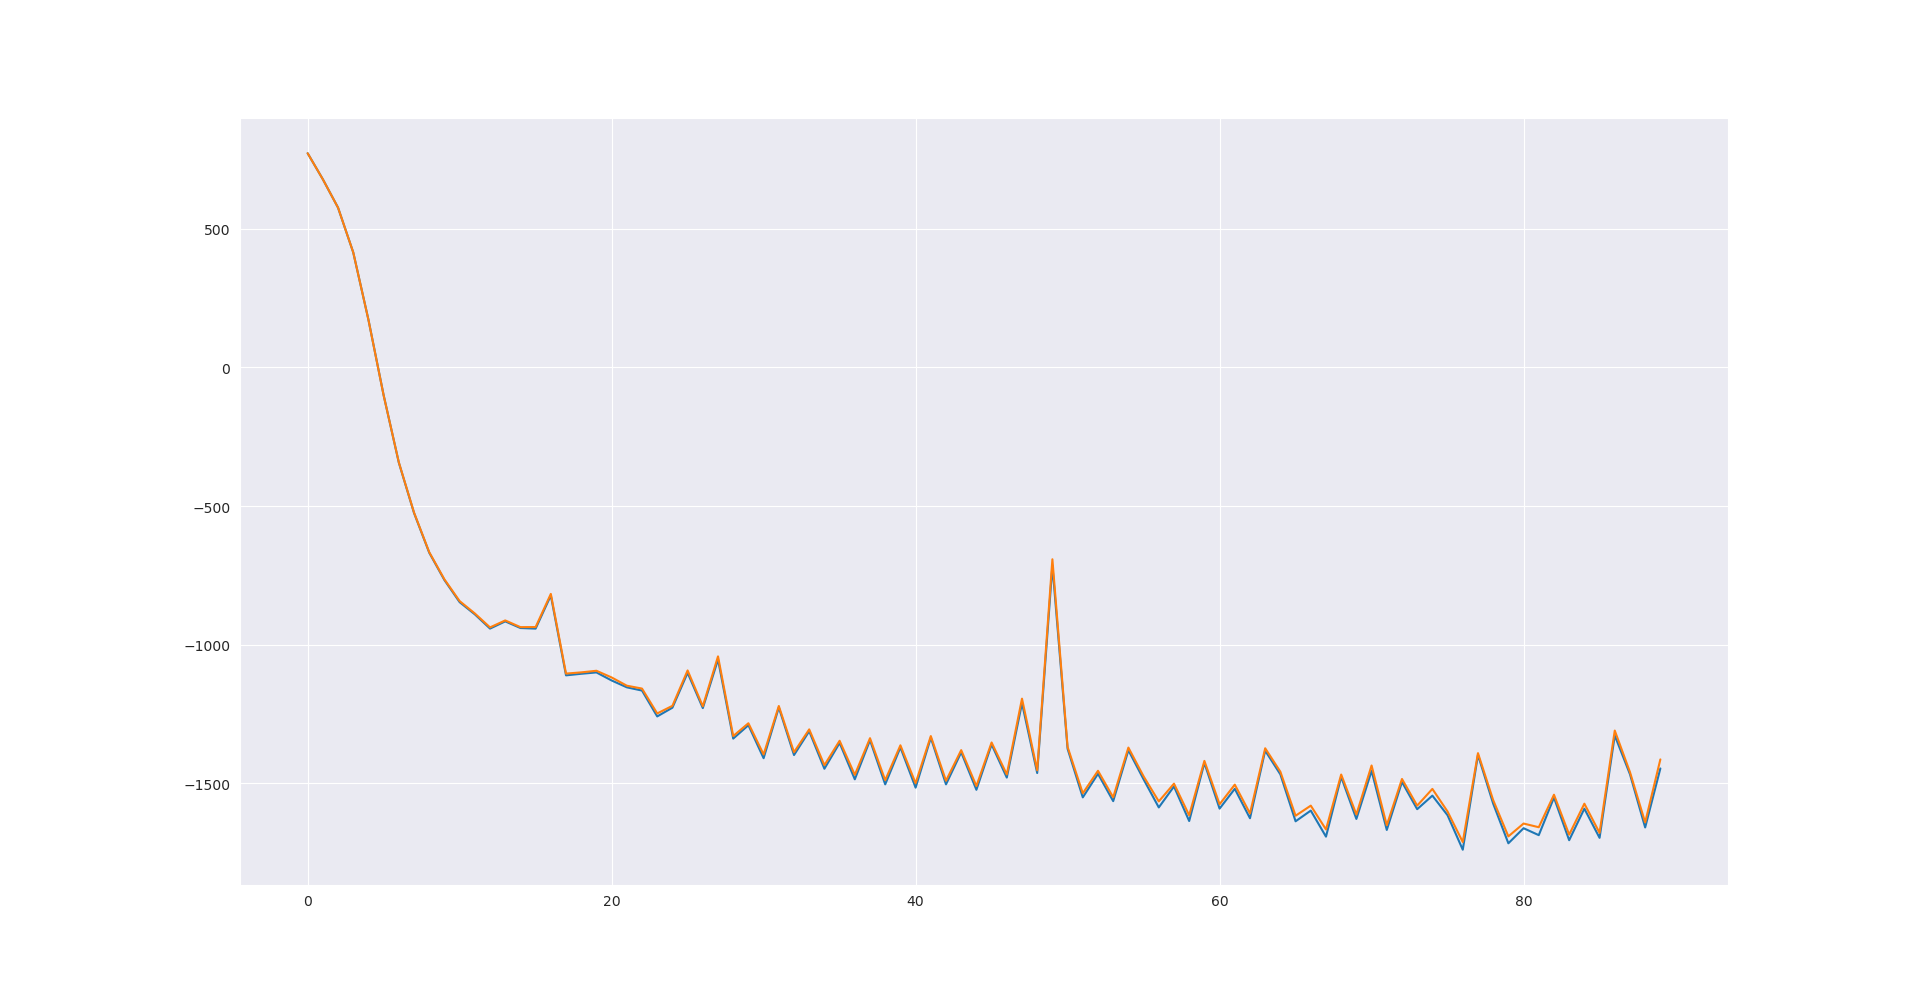
\includegraphics[width=\linewidth]{images/train_test_error.png}
    \caption{Training and validation error of the MNIST VAE.}
    \label{fig:train_test_error}
\end{figure}

Another way to check the correctness of the implementation was to visualize the reconstructed digits.
The expectation was that before the training we will see only the noise and after each epoch, the pictures will be approximating the original digits more and more.
Also, we expected the images to have blurry edges because of the standard deviation of the univariate normal distribution produced by the probabilistic decoder as an output.
These expectations were met, therefore we concluded that our implementation works correctly.
The improving reconstruction of the digits over the epochs is visualized in Figure \ref{fig:reconstruction}.

\begin{figure}
    \centering
    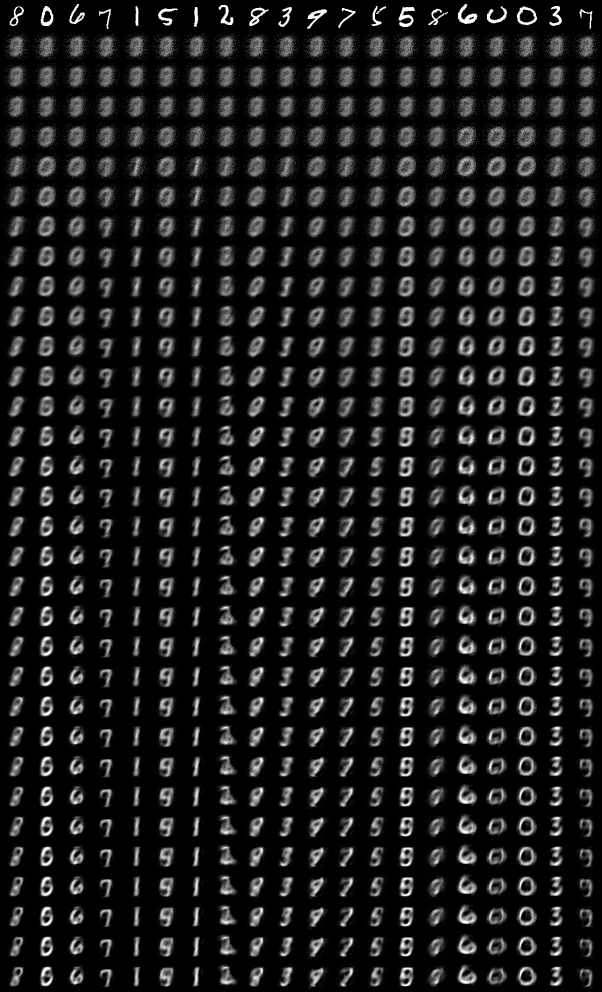
\includegraphics[width=\linewidth]{images/reconstruction_15.png}
    \caption{Reconstruction of the digits across the epochs.}
    \label{fig:reconstruction}
\end{figure}

% the reconstruction and interpretation of latent variables
\newpage
We were also curious about the interpretation of the latent space and therefore we constructed Figure \ref{fig:sample}.
In this visualization, we calculated the average representation of the digit three.
We did this by taking all $z_{\mu}$ representations and calculating the mean value of them.
Then we modified the $i$-th entry from the resulting vector and decoded this representation using the probabilistic decoder to produce the $i$-th row of the Figure \ref{fig:sample}.
This showed us what is the influence of the $i$-th entry on the generated picture.
As we can see, most of the entries did not produce something that we humans would consider meaningful, although for example increasing the 10-th entry reminds us of the digit nine.

In the literature, the representation which we got is sometimes also called entangled representation.
The disentangled representation would then be a representation, where changing a single factor in the learned representation would lead to a change of one factor in the original picture.
Variational autoencoders can be also used to search for disentangled representations  \cite{higgins2016disentangled}, but this is out of the scope of this project.

\begin{figure}
    \centering
    
\includegraphics[width=\linewidth]{images/sample.png}
    \caption{Visualization of the effect of the latent space on the decoded digit three}
    \label{fig:sample}
\end{figure}

\newpage
\section{CORTEX variational autoencoder}
% description of the dataset
The CORTEX dataset is a set of single-cell RNA-seq data from the mouse cerebral cortex cells.
The dataset consists of 3005 mouse cells labelled as 7 distinct cell types.
This dataset was used to illustrate the possibility of using the VAE on the single-cell RNA-seq data.

% scaling of the data
Because of the high number of dimensions we decided to use only the first 558 genes ordered by variance, similarly to the Publication \cite{lopez2018scvi}.
Further, we normalized the data using the column-wise min-max normalization the same way how we did with the MNIST dataset.

The variational autoencoder used for the modelling had almost the same architecture as described in the MNIST experiment.
The only difference was the size of the input to the probabilistic encoder and the output from the probabilistic decoder, which was 558 in this case instead of 784.

Since we used this architecture, we were allowed to use the same training process as well.
We also monitored the SGVB error for train and validation set and stopped the training, when the training and validation error diverged.
The error is visualized in the Figure \ref{fig:sc_error}.

\begin{figure}
    \centering
    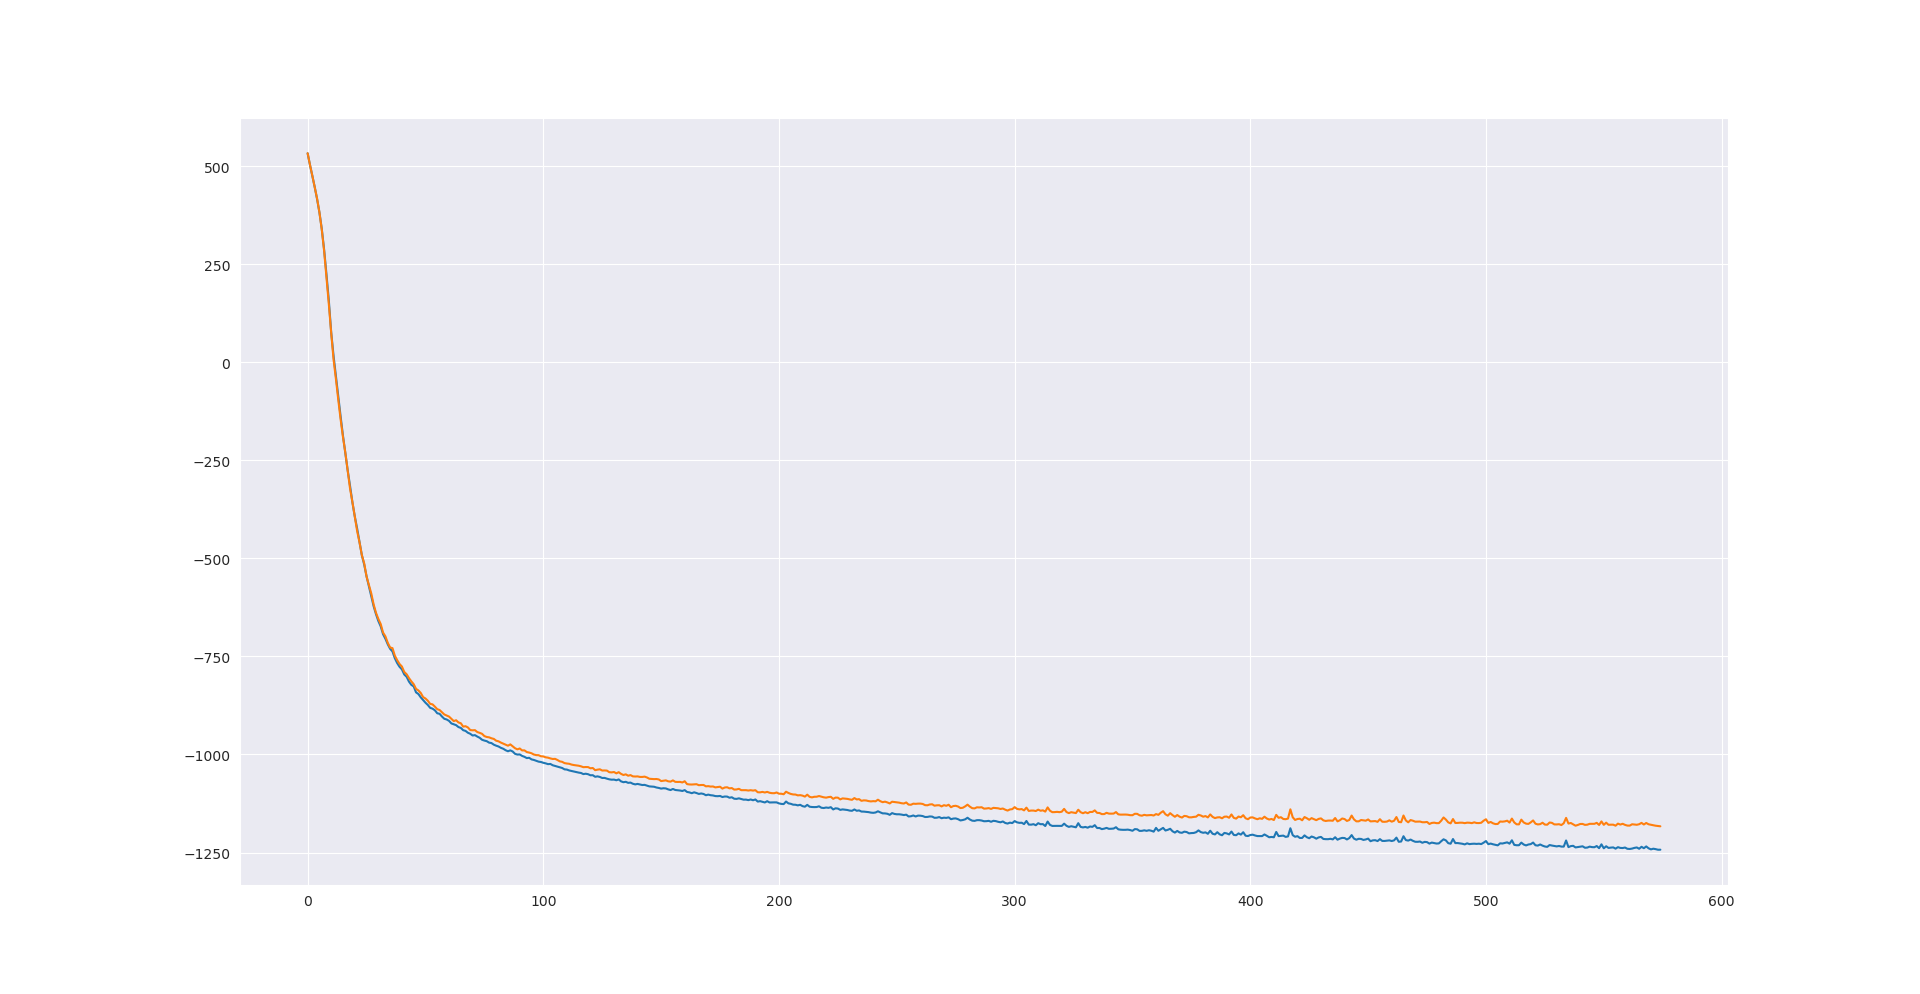
\includegraphics[width=\linewidth]{images/single_cell_training.png}
    \caption{Training and validation error for single-cell RNA-seq data.}
    \label{fig:sc_error}
\end{figure}

To demonstrate the usefulness of the latent representation generated from the variational autoencoder on the single-cell RNA-seq data, we visualized this 20-dimensional representation in two dimensions using the t-SNE.
We coloured the data points according to their corresponding labels as shown in Figure \ref{fig:cortex} (top).
The figure reveals that the variational autoencoder was able to learn a representation which can be used for clustering analysis.
We also provide an original visualization from the Publication \cite{lopez2018scvi} in the Figure \ref{fig:cortex} (bottom).
As we can see, we obtained similar clustering patterns, further confirming the correctness of these results.

\begin{figure}
    \centering
    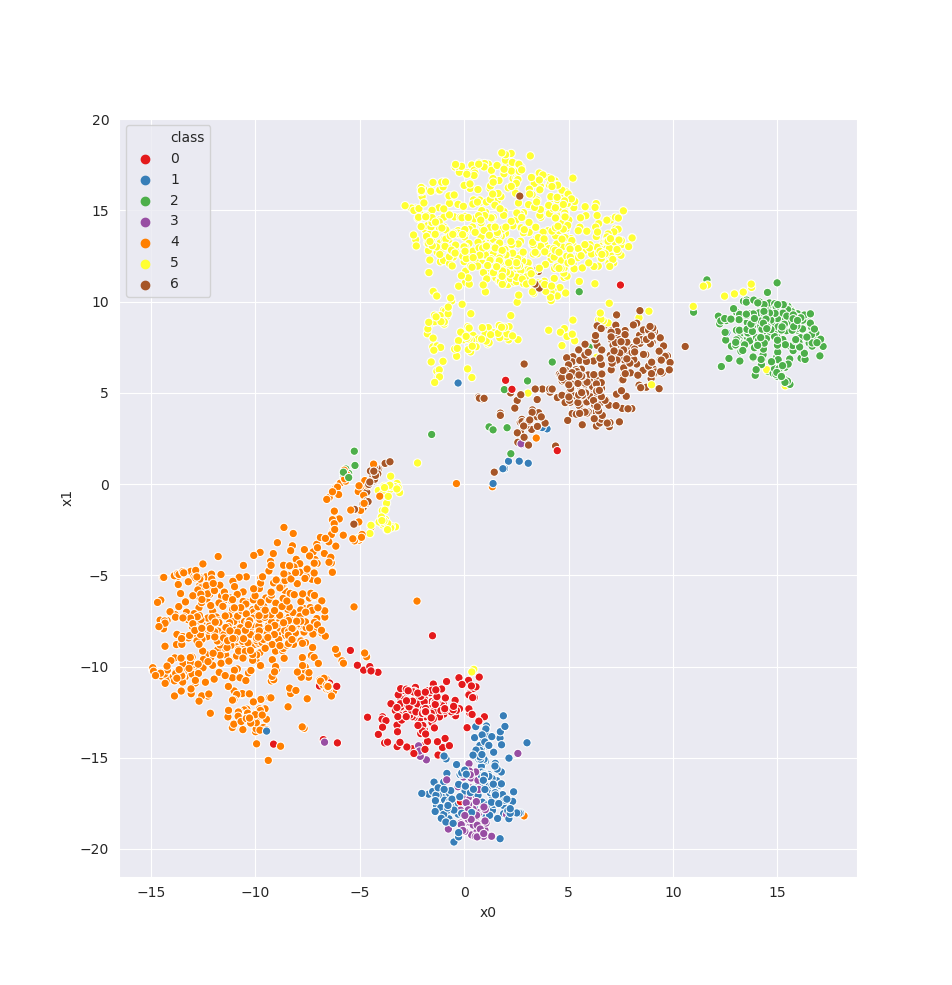
\includegraphics[width=\linewidth]{images/sc_data_VAE.png}
    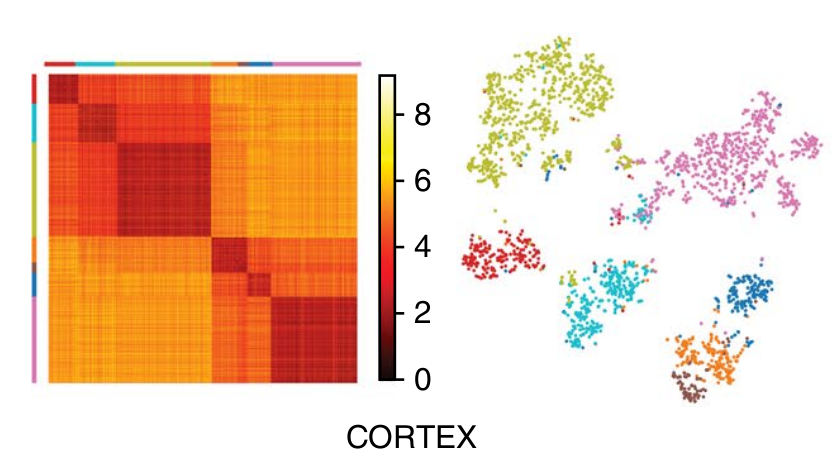
\includegraphics[width=\linewidth]{images/scVI_plot.png}
    \caption{t-SNE visualization of the latent representation of CORTEX dataset}
    \label{fig:cortex}
\end{figure}

% \chapter{Discussion}
% \label{chap:discuss}

% Is it possible to generalise?
% Make comparisons with other studies
% Are there alternative explanations?
% What are the strong and weak aspects of your paper?
% What are the practical implications?
% Is more research needed?
% Make recommendations (to be applied in practice).

\chapter{Conclusion}
\label{chap:conclusion}

The main goal of this project was to show how to use the variational autoencoders to create a low-dimensional probabilistic representation of the single-cell RNA-seq data.
One of the advantages of this representation for the downstream analysis tasks is the possibility to model the uncertainty of the data.
Another advantage of using the variational autoencoders is that they enable us to capture non-linear relationships between the data and the representation and that they provide a natural way to use them with recent big datasets.

Since the variational autoencoders are the combination of neural networks architecture with the variational inference, we needed to introduce these two topics.

In the part about the neural networks, we described the basic model, its components and how to train such a model using the Stochastic Gradient Descent method.
Then we showed how to apply these concepts for the standard autoencoder architecture and what are the main differences.

To explain the variational inference, we first needed to introduce the basic concepts from the Bayesian inference, since the variational inference is trying to approximate it.
To better illustrate the goal of the Bayesian inference, we showed an example of Approximate Bayesian Computation, as we think this is the simplest procedure to explain.
We also included a summary of MCMC methods, since these are the most commonly used methods for approximating the Bayesian inference and we wanted to highlight the main difference between MCMC methods and variational inference.
Finally, we described the variational inference in details.
We showed how to reformulate the original problem into an optimization problem and we introduced an ELBO quantity, which helped us to solve this problem.

At the end of the second chapter, we combined those two topics into variational autoencoder and explained how we can train this model.

In the implementation part of this project, we explain the details of the used architecture.
We also show, how we tested the correctness of our program with the MNIST dataset.
Finally, we demonstrated how to use the model on the single-cell RNA-seq CORTEX dataset and we compared the results with the results from the original publication.

\bibliographystyle{unsrt}
\bibliography{0_sources} 

\end{document}
